\documentclass[11pt]{preprint}

\setlength{\topmargin}{0mm} \setlength{\oddsidemargin}{0mm}
\setlength{\textwidth}{160mm} \setlength{\textheight}{215mm}

\usepackage{amssymb,amsmath,amscd,amsthm}
\usepackage{tikz}
\usepackage{wrapfig}

\newtheorem{proposition}{Proposition}

\def\enumb{\begin{enumerate}}
\def\enume{\end{enumerate}}
\def\integers{\mathbb{Z}}
\def\multiset#1#2{\ensuremath{\left(\kern-.3em\left(\genfrac{}{}{0pt}{}{#1}{#2}\right)\kern-.3em\right)}}

\title{Discrete Mathematics, 2016 Spring - HW 13}
\author{Instructor: Zsolt Pajor-Gyulai}
\institute{Courant Institute of Mathematical Sciences, NYU}



\begin{document}

\maketitle

To get full credit  in all of the problems, use rigorous justification and unless otherwise indicated, make sure that your solution reads as a perfect English sentence. You should only assume integers, operations and order relations as given. If you use a statement or a definition from the textbook, make sure to indicate it.
\vspace{0.2cm}

\textbf{Section 44}
\enumb
\item[4)] Let's assume Alice and Bob both have public encryption functions $E_A$ and $E_B$, respectively, and closely guarded, private decryption functions $D_A$ and $D_B$. Alice and Bob each know the other's public function, and presumably Eve knows $E_A$ and $E_B$ too.

%Normally, when Alice wants to send a message $M$ to Bob, she encrypts the message with Bob's public function $E_B$, transmits $E_B(M)$ to Bob, and he decrypts with his private function $D_B$ by computing $D_B(E_B(M))=M$.

Here is an alternative way  to the protocol we learned about in class Alice can use. She first encrypts the message $M$ by computing $D_A(M)$ and then sends the result to Bob. Let's explore the implications of her following this alternative protocol.
\enumb
\item Alice has sent $D_A(M)$ to Bob. How does he recover the original message $M$?
\item Eve intercepts the transmission $D_A(M)$. Can she also decrypt this message?
\item The message Alice sent to Bob was nasty and she tries to claim that Eve sent the message. How does Eve defend herself?
\enume
The point of $(c)$ is that Alice cannot deny having sent the message; in that sense, she has put her digital signature on the message.
\enume

\textbf{Section 47}
\enumb
\item[1)] The following pictures represent graphs. Please write each of these graphs as a pair of sets $(V,E)$.
\begin{figure}[ht]
\centering
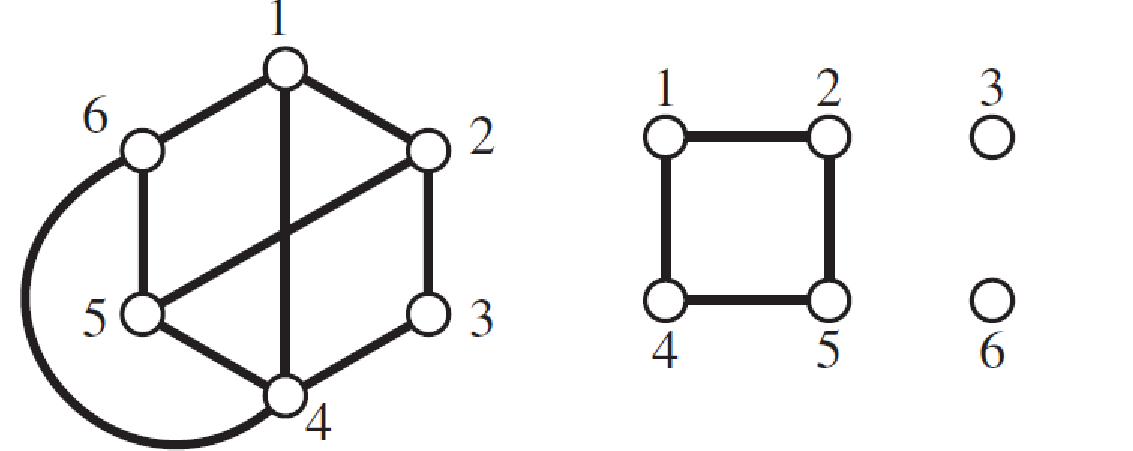
\includegraphics[scale=0.4]{Graphs1.pdf}
\end{figure}


\item[2)] Draw pictures of the following graphs.
\enumb
\item $\left(\{a,b,c,d,e\},\left\{\{a,b\},\{a,c\},\{b,c\},\{b,d\},\{c,d\}\right\}\right)$
\item $\left(\{a,b,c,d,e\},\left\{\{a,c\},\{b,d\},\{b,e\}\right\}\right)$
\enume
\item[15)] Let $G$ be a simple graph. Prove that there must be an even number of vertices with odd degree.
\item[16)] Prove that in any graph with two or more vertices, there must be two vertices of the same degree.
\enume

\textbf{Section 48}

\enumb
\item[5)] Let $G$ be the graph in the picture.
\begin{figure}[ht]
\centering
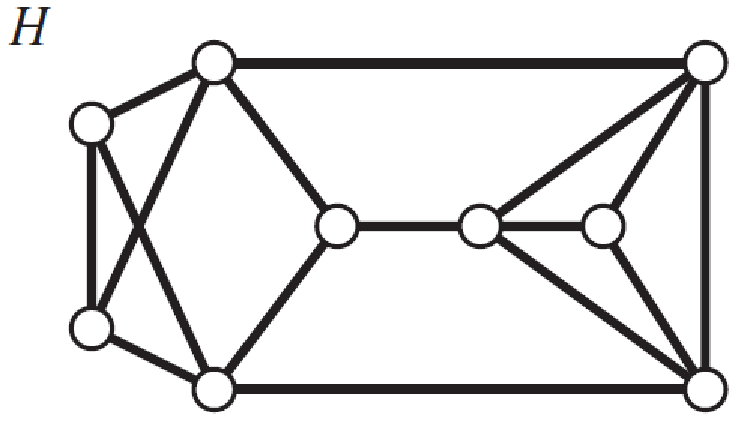
\includegraphics[scale=0.4]{Graphs2.pdf}
\end{figure}
\enumb
\item Draw the complement graph $\bar{G}$.
\item Find $\alpha(G)$ and $\omega(G)$.
\enume
\item[12)] This problem is in connection with Proposition 48.13 on p342. Find a graph on five vertices for which $\omega(G)<3$ and $\omega(\bar{G})<3$. This shows that the number six in the proposition is the best possible.
\enume


\end{document}